\documentclass[conference]{IEEEtran}

\usepackage[T1]{fontenc}
\usepackage[utf8]{inputenc}
\usepackage{cite}
\usepackage{graphicx}
\usepackage{booktabs}
\usepackage{array}
\usepackage{multirow}
\usepackage{url}
\usepackage{xcolor}
\usepackage{listings}
\usepackage{tikz}
\usepackage{hyperref}
\usepackage{enumitem}
\usepackage{amsmath}

\usetikzlibrary{arrows.meta,positioning,shapes.geometric,fit,backgrounds}

\hypersetup{
  colorlinks=true,
  linkcolor=blue,
  urlcolor=blue,
  citecolor=blue
}

\lstdefinestyle{smallcode}{
  basicstyle=\ttfamily\footnotesize,
  breaklines=true,
  frame=single,
  columns=fullflexible
}

\title{Roadlytics: Engineering Report for a Web-Based Road Intelligence Platform}

\author{
\IEEEauthorblockN{Prepared for the Roadlytics Project}
\IEEEauthorblockA{
Repository: Hammadullah2/Roadlytics \\
Deployment branch used during cloud rollout: \texttt{version2} \\
Report revision reference: commit \texttt{039d705}
}
}

\begin{document}
\maketitle

\begin{abstract}
This report documents the design, implementation, deployment, and validation of
\textbf{Roadlytics}, a web-based remote-sensing application for road
segmentation, road-condition classification, and connectivity analytics from
Sentinel-2 imagery. The platform converts an existing research-oriented
\texttt{road\_pipeline} codebase into an operational system composed of a
Next.js frontend, a FastAPI backend, an asynchronous inference worker, Docker
deployment assets, Azure Blob storage integration, and an Azure-hosted virtual
machine runtime. The report covers the problem definition, end-to-end user
workflow, software architecture, deployment topology, data flow, technology
stack, operational incidents encountered during deployment, and the engineering
changes required to make the system cloud-executable. It also records major
deployment challenges including Azure region restrictions, quota limitations,
Caddy reverse-proxy misconfiguration, direct-to-blob browser CORS behavior, SSH
key permission issues on Windows, and a backend queue recovery bug affecting
jobs after service restarts.
\end{abstract}

\begin{IEEEkeywords}
Road analytics, Sentinel-2, GeoTIFF, FastAPI, Next.js, Docker, Azure Blob,
geospatial AI, road segmentation, road condition classification
\end{IEEEkeywords}

\section{Introduction}
Roadlytics was conceived as a full-stack operationalization of an existing
geospatial machine learning pipeline. The original logic was organized around a
folder named \texttt{road\_pipeline}, containing the core domain logic for road
segmentation and road-condition classification. The project goal was to
transform this pipeline into a browser-accessible application where a user can:

\begin{enumerate}[leftmargin=16pt]
\item upload a four-band Sentinel-2 Level-2 GeoTIFF in the expected band order
\texttt{B2/B3/B4/B8},
\item select a segmentation method from \texttt{DeepLabV3} or \texttt{PakOSM},
\item select a condition-classification method from \texttt{KMeans} or
\texttt{EfficientNet},
\item execute the pipeline in the cloud,
\item inspect outputs on a map overlaid on top of the original Sentinel image
and an OpenStreetMap base layer, and
\item download generated rasters, analytics outputs, reports, and shapefiles.
\end{enumerate}

The implementation effort therefore included both productization and system
engineering. The work expanded beyond simply exposing inference endpoints: it
required storage abstraction, job orchestration, tiling for map visualization,
frontend workflow design, Docker packaging, Azure deployment assets, and runtime
resilience improvements.

\section{Project Objectives}
The primary objectives of the implementation were:

\begin{itemize}[leftmargin=16pt]
\item preserve the scientific workflow already encoded in
\texttt{road\_pipeline},
\item expose the workflow through a web application suitable for non-technical
users,
\item support two segmentation options and two classification options without
changing the user upload flow,
\item generate final road-condition masks using a fixed semantic color scheme:
good = green, unpaved = red, damaged = yellow,
\item compute raster-first connectivity analytics from segmentation and
classification outputs,
\item deploy the system on a low-cost Azure virtual machine using Docker, and
\item maintain a path for future hardening, scaling, and model upgrades.
\end{itemize}

\section{System Scope}
Roadlytics Phase 1 includes the following functional scope:

\begin{itemize}[leftmargin=16pt]
\item upload initialization and file ingest,
\item job registration and background execution,
\item Sentinel-2 validation,
\item road segmentation,
\item road-condition classification,
\item connectivity analysis,
\item artifact packaging,
\item map-based overlay analysis,
\item HTML reporting, and
\item download access to generated outputs.
\end{itemize}

The system intentionally omits authentication, role-based administration,
multi-tenant isolation, and distributed job scheduling in this initial release.

\section{Overall Architecture}
Roadlytics was implemented as a three-layer product system built around the
original ML pipeline.

\begin{figure*}[t]
\centering
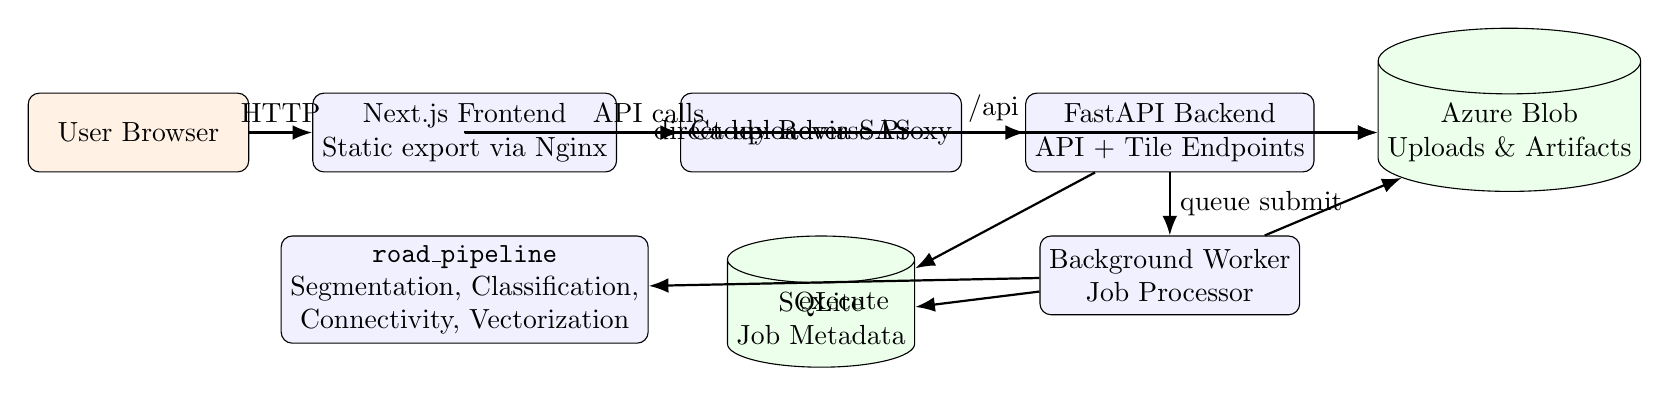
\begin{tikzpicture}[
  node distance=8mm and 8mm,
  box/.style={draw, rounded corners, align=center, minimum width=28mm, minimum height=10mm, fill=gray!8},
  service/.style={draw, rounded corners, align=center, minimum width=30mm, minimum height=10mm, fill=blue!6},
  store/.style={draw, cylinder, shape border rotate=90, aspect=0.25, align=center, minimum height=14mm, minimum width=18mm, fill=green!8},
  flow/.style={-{Latex[length=2.5mm]}, thick}
]
\node[box, fill=orange!10] (user) {User Browser};
\node[service, right=of user] (frontend) {Next.js Frontend\\Static export via Nginx};
\node[service, right=of frontend] (caddy) {Caddy Reverse Proxy};
\node[service, right=of caddy] (backend) {FastAPI Backend\\API + Tile Endpoints};
\node[service, below=of backend] (worker) {Background Worker\\Job Processor};
\node[service, below=of frontend] (pipeline) {\texttt{road\_pipeline}\\Segmentation, Classification,\\Connectivity, Vectorization};
\node[store, below=of caddy] (sqlite) {SQLite\\Job Metadata};
\node[store, right=of backend] (blob) {Azure Blob\\Uploads \& Artifacts};

\draw[flow] (user) -- node[above] {HTTP} (frontend);
\draw[flow] (frontend) -- node[above] {API calls} (caddy);
\draw[flow] (caddy) -- node[above] {/api} (backend);
\draw[flow] (backend) -- node[right] {queue submit} (worker);
\draw[flow] (worker) -- node[below] {execute} (pipeline);
\draw[flow] (backend) -- (sqlite);
\draw[flow] (worker) -- (sqlite);
\draw[flow] (backend) -- (blob);
\draw[flow] (worker) -- (blob);
\draw[flow] (frontend) |- node[pos=0.75, left] {direct upload\\via SAS} (blob);
\end{tikzpicture}
\caption{High-level logical architecture of Roadlytics.}
\label{fig:architecture}
\end{figure*}

The core architectural layers are:

\begin{enumerate}[leftmargin=16pt]
\item \textbf{Frontend layer}: a Next.js application rendered as a static export
and served from an Nginx container.
\item \textbf{Application layer}: a FastAPI backend exposing upload, job,
artifact, report, analytics, and map-tile endpoints.
\item \textbf{Execution layer}: a background worker that runs the original
\texttt{road\_pipeline} modules in a job-oriented manner.
\end{enumerate}

The application uses:

\begin{itemize}[leftmargin=16pt]
\item Azure Blob Storage for uploaded inputs and generated artifacts,
\item SQLite for metadata and job tracking on the VM,
\item Docker Compose for orchestration on the VM, and
\item Caddy as the reverse proxy for frontend/backend routing.
\end{itemize}

\section{End-to-End Workflow}
The operational workflow implemented in Roadlytics is illustrated in
Fig.~\ref{fig:pipelineflow}.

\begin{figure*}[t]
\centering
\begin{tikzpicture}[
  node distance=6mm and 7mm,
  step/.style={draw, rounded corners, align=center, minimum width=25mm, minimum height=10mm, fill=gray!8},
  choice/.style={draw, diamond, aspect=2, align=center, inner sep=1pt, fill=orange!8},
  flow/.style={-{Latex[length=2.5mm]}, thick}
]
\node[step] (upload) {Upload Sentinel-2\\4-band GeoTIFF};
\node[step, right=of upload] (validate) {Validate raster\\bands and metadata};
\node[choice, right=of validate, xshift=2mm] (segchoice) {Segmentation\\choice};
\node[step, above right=of segchoice] (deeplab) {DeepLabV3\\road mask};
\node[step, below right=of segchoice] (pakosm) {PakOSM\\road mask};
\node[choice, right=28mm of segchoice] (clschoice) {Classification\\choice};
\node[step, above right=of clschoice] (eff) {EfficientNet\\condition masks};
\node[step, below right=of clschoice] (kmeans) {KMeans\\condition masks};
\node[step, right=of clschoice, xshift=30mm] (conn) {Connectivity\\analytics};
\node[step, right=of conn] (package) {Artifacts, tiles,\\report, shapefiles};
\node[step, right=of package] (ui) {Map analysis\\and downloads};

\draw[flow] (upload) -- (validate);
\draw[flow] (validate) -- (segchoice);
\draw[flow] (segchoice) -- (deeplab);
\draw[flow] (segchoice) -- (pakosm);
\draw[flow] (deeplab.east) |- (clschoice.north west);
\draw[flow] (pakosm.east) |- (clschoice.south west);
\draw[flow] (clschoice) -- (eff);
\draw[flow] (clschoice) -- (kmeans);
\draw[flow] (eff.east) |- (conn.north west);
\draw[flow] (kmeans.east) |- (conn.south west);
\draw[flow] (conn) -- (package);
\draw[flow] (package) -- (ui);
\end{tikzpicture}
\caption{Operational pipeline flow implemented in Roadlytics.}
\label{fig:pipelineflow}
\end{figure*}

The detailed execution path is as follows:

\begin{enumerate}[leftmargin=16pt]
\item The user uploads a Sentinel-2 GeoTIFF from the Projects page.
\item The frontend requests an upload session from the backend.
\item In Azure mode, the backend returns a Blob SAS URL; the browser uploads the
file directly to Azure Blob.
\item The frontend creates a job referencing the uploaded blob.
\item The backend persists the job to SQLite and submits it to the worker queue.
\item The worker downloads the raster, validates the expected format, and
generates a display RGB raster.
\item The selected segmentation path generates a road mask.
\item The selected classification path generates three class masks and one
combined condition raster.
\item Connectivity analysis computes components, a weighted criticality surface,
summary statistics, and a critical junction output.
\item Packaging generates web-display rasters, shapefile archives, HTML reports,
and artifact metadata.
\item The frontend polls the job endpoint until the run is complete and then
loads results on the map and reporting pages.
\end{enumerate}

\section{User Flow}
The web product was shaped around a simple browser-first operational flow, shown
in Fig.~\ref{fig:userflow}.

\begin{figure}[t]
\centering
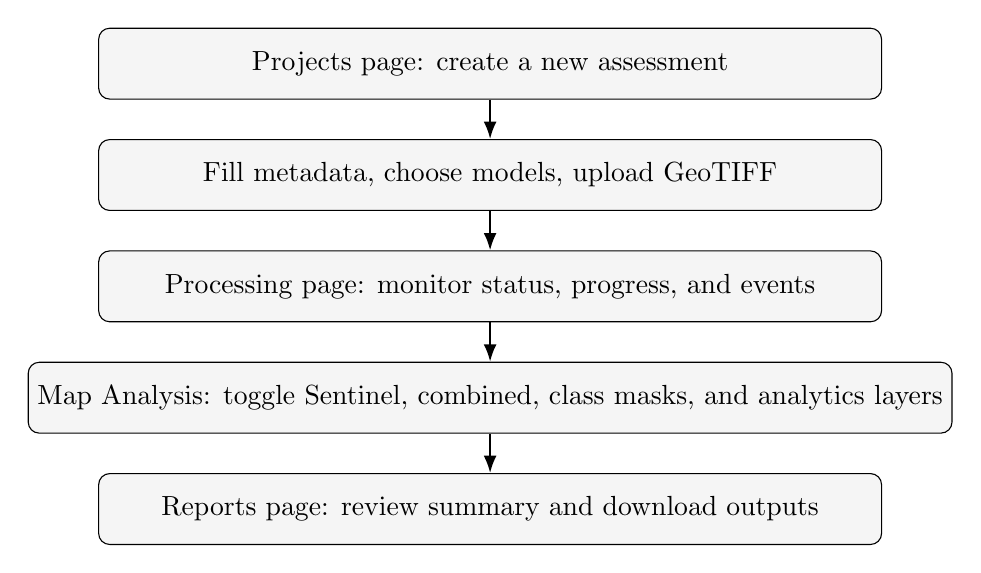
\begin{tikzpicture}[
  node distance=5mm,
  uf/.style={draw, rounded corners, align=center, minimum width=0.82\columnwidth, minimum height=9mm, fill=gray!8},
  flow/.style={-{Latex[length=2.2mm]}, thick}
]
\node[uf] (projects) {Projects page: create a new assessment};
\node[uf, below=of projects] (upload) {Fill metadata, choose models, upload GeoTIFF};
\node[uf, below=of upload] (processing) {Processing page: monitor status, progress, and events};
\node[uf, below=of processing] (map) {Map Analysis: toggle Sentinel, combined, class masks, and analytics layers};
\node[uf, below=of map] (reports) {Reports page: review summary and download outputs};

\draw[flow] (projects) -- (upload);
\draw[flow] (upload) -- (processing);
\draw[flow] (processing) -- (map);
\draw[flow] (map) -- (reports);
\end{tikzpicture}
\caption{Primary user flow in the web application.}
\label{fig:userflow}
\end{figure}

The user experience centers around five product areas:

\begin{itemize}[leftmargin=16pt]
\item \textbf{Dashboard}: summary and navigation surface.
\item \textbf{Projects}: assessment creation and project library.
\item \textbf{Processing}: stage monitoring and event timeline.
\item \textbf{Map Analysis}: geospatial result inspection with layer toggles.
\item \textbf{Reports}: HTML report review and artifact export.
\end{itemize}

\section{Road Pipeline Refactoring}
The original \texttt{road\_pipeline} codebase was preserved as the domain engine,
but it was refactored and integrated in a service-oriented manner. The
application-level job processor now imports and orchestrates the following
components directly:

\begin{itemize}[leftmargin=16pt]
\item \texttt{road\_pipeline.segmentation.deeplabv3}
\item \texttt{road\_pipeline.segmentation.osm\_to\_mask}
\item \texttt{road\_pipeline.classification.efficientnet}
\item \texttt{road\_pipeline.classification.kmeans}
\item \texttt{road\_pipeline.analytics.connectivity}
\item \texttt{road\_pipeline.postprocess.raster\_to\_vector}
\end{itemize}

Several important implementation requirements were added around the original
pipeline:

\begin{itemize}[leftmargin=16pt]
\item consistent per-job work directories,
\item artifact registration and storage upload,
\item color-correct condition masks,
\item display-optimized raster outputs,
\item HTML report generation,
\item packageable shapefile archives, and
\item integration with the web map tiling layer.
\end{itemize}

\subsection{Semantic Raster Output Scheme}
The user requested a fixed semantic coloring convention. The implementation now
uses:

\begin{itemize}[leftmargin=16pt]
\item \textbf{good roads}: green,
\item \textbf{unpaved roads}: red,
\item \textbf{damaged roads}: yellow,
\item \textbf{combined raster}: palette-coded raster containing all classes.
\end{itemize}

This change was important because the downstream map experience depends on the
colors being understandable immediately by non-technical users.

\subsection{Raster-First Connectivity Analytics}
Phase 1 explicitly required a raster-first Stage 5 rather than a graph built
from shapefiles. The implemented connectivity stage uses:

\begin{itemize}[leftmargin=16pt]
\item the segmentation mask raster,
\item the combined classification raster,
\item a weighted cost map using class-aware traversal costs,
\item connected-component extraction,
\item betweenness-inspired criticality output, and
\item critical junction export to GeoJSON.
\end{itemize}

Produced artifacts include:

\begin{itemize}[leftmargin=16pt]
\item \texttt{component\_map.tif},
\item \texttt{betweenness\_centrality.tif},
\item \texttt{connected\_components.csv},
\item \texttt{analytics\_summary.json},
\item \texttt{critical\_junctions.geojson}.
\end{itemize}

\section{Backend Design}
The backend is a FastAPI application running in a Python 3.11 container. It
owns all orchestration responsibilities other than frontend rendering.

\subsection{Backend Responsibilities}
The backend is responsible for:

\begin{itemize}[leftmargin=16pt]
\item upload initialization,
\item local-proxy upload fallback,
\item job creation and job-state polling,
\item artifact and layer serialization,
\item report serving,
\item tile endpoint exposure,
\item background-worker startup,
\item database initialization, and
\item storage backend selection.
\end{itemize}

\subsection{REST Endpoints}
The public interface includes the following route families:

\begin{itemize}[leftmargin=16pt]
\item \texttt{/api/uploads/init}
\item \texttt{/api/uploads/\{upload\_id\}/file}
\item \texttt{/api/jobs}
\item \texttt{/api/jobs/\{job\_id\}}
\item \texttt{/api/jobs/\{job\_id\}/artifacts}
\item \texttt{/api/jobs/\{job\_id\}/analytics}
\item \texttt{/api/jobs/\{job\_id\}/report}
\item tile routes for layer rendering
\end{itemize}

\subsection{Persistence Model}
SQLite was selected for the first deployment because the system initially runs
on a single Azure VM and does not require distributed consistency. The schema
contains:

\begin{itemize}[leftmargin=16pt]
\item \texttt{jobs}: job identity, stage, status, progress, and metadata,
\item \texttt{artifacts}: output descriptors and display-layer information,
\item \texttt{job\_events}: user-visible processing timeline,
\item \texttt{analytics\_snapshots}: summary analytics payloads.
\end{itemize}

\section{Frontend Design}
The frontend is a Next.js application, statically exported and served by Nginx.
It consumes the backend entirely through HTTP APIs and layer URLs.

\subsection{Frontend Responsibilities}
The frontend is responsible for:

\begin{itemize}[leftmargin=16pt]
\item project creation UX,
\item upload initiation,
\item polling job status,
\item presenting stage progress,
\item loading raster and vector layers on the map,
\item exposing report and download links,
\item preserving a clear operator workflow.
\end{itemize}

\subsection{Map Layering Model}
The map stack follows the requested visual order:

\begin{enumerate}[leftmargin=16pt]
\item OpenStreetMap base layer, always visible,
\item Sentinel RGB upload raster,
\item combined condition mask,
\item individual class masks,
\item connectivity analysis layers,
\item critical junctions vector layer.
\end{enumerate}

The OSM tile URL was made configurable through frontend environment variables to
avoid hard-coding a single tile source permanently.

\section{Cloud Deployment Topology}
The deployment uses Docker Compose on a single Azure Ubuntu VM. The topology is
shown in Fig.~\ref{fig:deployment}.

\begin{figure}[t]
\centering
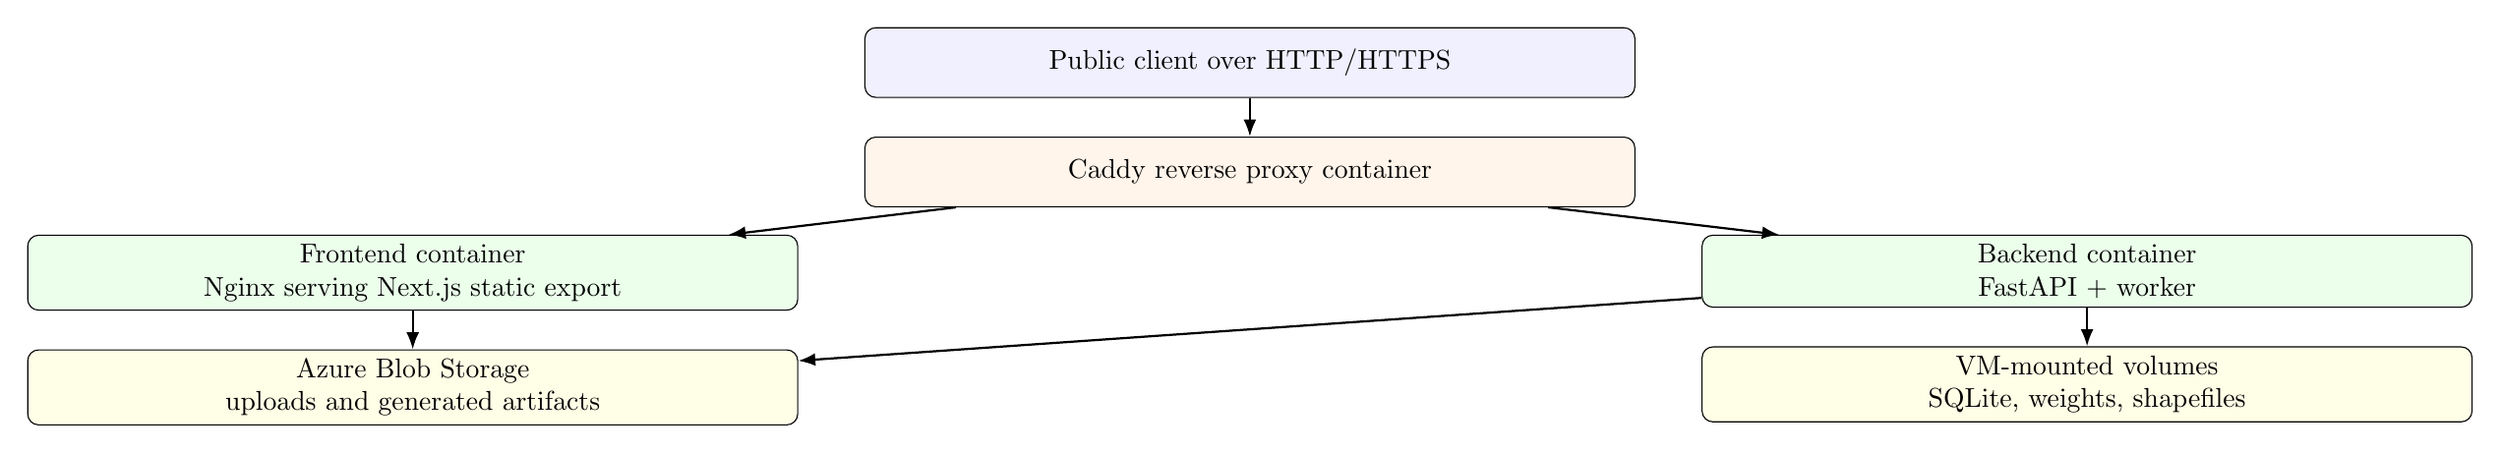
\begin{tikzpicture}[
  node distance=5mm,
  box/.style={draw, rounded corners, align=center, minimum width=0.82\columnwidth, minimum height=9mm, fill=gray!8},
  flow/.style={-{Latex[length=2.2mm]}, thick}
]
\node[box, fill=blue!6] (internet) {Public client over HTTP/HTTPS};
\node[box, below=of internet, fill=orange!8] (caddy) {Caddy reverse proxy container};
\node[box, below left=of caddy, xshift=-5mm, fill=green!8] (frontend) {Frontend container\\Nginx serving Next.js static export};
\node[box, below right=of caddy, xshift=5mm, fill=green!8] (backend) {Backend container\\FastAPI + worker};
\node[box, below=of backend, fill=yellow!10] (vmfs) {VM-mounted volumes\\SQLite, weights, shapefiles};
\node[box, below=of frontend, fill=yellow!10] (blob) {Azure Blob Storage\\uploads and generated artifacts};

\draw[flow] (internet) -- (caddy);
\draw[flow] (caddy) -- (frontend);
\draw[flow] (caddy) -- (backend);
\draw[flow] (backend) -- (vmfs);
\draw[flow] (backend) -- (blob);
\draw[flow] (frontend) -- (blob);
\end{tikzpicture}
\caption{Deployment topology on the Azure VM.}
\label{fig:deployment}
\end{figure}

\subsection{Containers}
The deployment consists of:

\begin{itemize}[leftmargin=16pt]
\item \textbf{frontend}: Next.js build output served by Nginx,
\item \textbf{backend}: FastAPI application and background worker in one
container,
\item \textbf{caddy}: reverse proxy and request router.
\end{itemize}

\subsection{Runtime Mounts}
The backend container mounts:

\begin{itemize}[leftmargin=16pt]
\item \texttt{./backend/data} for SQLite and working data,
\item \texttt{./model\_weights} for model weights,
\item \texttt{./data/osm\_roads} for PakOSM shapefiles.
\end{itemize}

\subsection{Azure Shape}
The deployed cloud shape is:

\begin{itemize}[leftmargin=16pt]
\item one Azure VM in East Asia,
\item one Azure Storage Account,
\item one private Blob container named \texttt{roadlytics},
\item Docker Compose as the orchestrator.
\end{itemize}

\section{Technology Stack}
Table~\ref{tab:stack} summarizes the major technologies used.

\begin{table*}[t]
\centering
\caption{Roadlytics technology stack.}
\label{tab:stack}
\begin{tabular}{p{32mm} p{42mm} p{88mm}}
\toprule
\textbf{Layer} & \textbf{Technology} & \textbf{Role} \\
\midrule
Frontend & Next.js, TypeScript, React, Nginx & Static web application, project creation flow, processing dashboard, map analysis, reports \\
Backend API & FastAPI, Pydantic, Uvicorn & REST API, upload initialization, job orchestration, report delivery, layer metadata \\
Background execution & Python worker service with asyncio queue & Asynchronous execution of long-running geospatial ML jobs \\
Geospatial/ML pipeline & \texttt{road\_pipeline}, PyTorch-based models, raster/vector processing libraries & Segmentation, classification, connectivity analytics, vectorization \\
Storage & Azure Blob Storage & Input upload storage and generated artifact storage \\
Database & SQLite & Persistent job state, artifacts, events, analytics summaries \\
Mapping & Leaflet/OpenStreetMap tile layer & Basemap and web layer composition \\
Containerization & Docker, Docker Compose & Build, runtime packaging, service orchestration \\
Proxy & Caddy & Reverse proxying between public entrypoint and internal containers \\
Cloud compute & Azure VM (Ubuntu) & Application host for the Docker stack \\
Deployment scripts & Bash, Compose overlay files & VM bootstrap, PakOSM fetch, production deployment \\
\bottomrule
\end{tabular}
\end{table*}

\section{Operational Challenges and Resolutions}
Several real deployment and runtime issues were encountered. These were not
hypothetical; they emerged during cloud bring-up and affected the execution
path.

\subsection{Azure Region Policy Restrictions}
An Azure policy blocked deployment attempts in unsupported regions. The initial
plan used Southeast Asia, but the subscription-exposed region list and actual VM
quota constraints required an East Asia deployment for compute. This required:

\begin{itemize}[leftmargin=16pt]
\item checking the effective region list from the portal,
\item aligning resource creation to allowed regions,
\item adapting deployment planning around subscription limitations.
\end{itemize}

\subsection{Azure VM Quota Limits}
The preferred D-series VM family was unavailable due to zero approved quota in
the attempted region. This forced a move to a smaller B-series machine
(\texttt{Standard B2as v2}), which is suitable for smoke testing but not ideal
for heavy CPU-based inference.

\subsection{Windows SSH Key Permissions}
The generated private key could not initially be used because Windows OpenSSH
rejected it as too broadly readable. The file ACLs had to be restricted so only
the owner retained read access.

\subsection{Caddy Startup Failure}
The reverse proxy initially failed repeatedly because the \texttt{encode}
directive was placed in the wrong part of the Caddyfile. After log inspection,
the configuration was corrected so \texttt{encode zstd gzip} appeared inside the
site block instead of the global block.

\subsection{Blob Upload Cross-Origin Behavior}
The first web upload attempt failed with a frontend \texttt{Failed to fetch}
error. Analysis showed that the browser upload path used direct Azure Blob SAS
uploads, which require proper Blob service CORS configuration for the frontend
origin.

\subsection{Input Validation Failure}
One early uploaded TIFF failed validation with the message that the Sentinel
upload must be a four-band GeoTIFF in \texttt{B2, B3, B4, B8} order. This
confirmed that validation logic was functioning and helped distinguish bad input
data from system-level failures.

\subsection{Queued Job Loss After Backend Restart}
The most important runtime bug discovered during testing was that jobs could
remain in the database with:

\begin{itemize}[leftmargin=16pt]
\item \texttt{status = queued},
\item \texttt{stage = uploaded},
\item \texttt{started\_at = NULL},
\end{itemize}

while never actually processing. The root cause was architectural: the worker
queue was held only in memory. If the backend container restarted after job
creation, the live queue was lost even though the jobs remained persisted in
SQLite.

The fix was to add a startup recovery routine so the backend re-queues
recoverable jobs from the database when the application starts. This change was
committed to branch \texttt{version2} as commit \texttt{039d705}.

\section{Key Engineering Outcomes}
The implementation produced the following major outcomes:

\begin{itemize}[leftmargin=16pt]
\item a browser-based Roadlytics application replacing a manual pipeline-only
workflow,
\item a cloud-deployable Docker runtime,
\item a geospatial results viewer with overlay toggles,
\item Azure Blob integration for inputs and artifacts,
\item packaged reports and downloadable outputs,
\item a documented Azure VM deployment path,
\item a resilience improvement for queue recovery after backend restart.
\end{itemize}

\section{Current Limitations}
Despite substantial progress, the current Roadlytics release still has several
known limitations:

\begin{itemize}[leftmargin=16pt]
\item no authentication or user isolation,
\item a single-node worker model,
\item SQLite persistence on a single VM,
\item limited observability beyond logs and database inspection,
\item constrained inference performance on the selected B-series VM,
\item dependence on correct Sentinel band ordering from the input file,
\item no autoscaling or distributed job executor.
\end{itemize}

\section{Recommended Next Steps}
The most valuable next engineering steps are:

\begin{enumerate}[leftmargin=16pt]
\item upgrade the VM or move the inference backend to stronger compute,
\item separate API and worker processes for clearer operational control,
\item introduce structured job retry semantics,
\item replace SQLite with a managed database if concurrency increases,
\item add authentication and project ownership,
\item add richer monitoring and health instrumentation,
\item optionally move the frontend to Azure Blob static hosting while keeping the
backend on the VM,
\item create a proper domain and enable production HTTPS.
\end{enumerate}

\section{Conclusion}
Roadlytics is no longer just a research folder containing isolated ML scripts.
It has been transformed into a deployable full-stack geospatial application with
real browser interaction, backend orchestration, map visualization, artifact
management, and cloud runtime infrastructure. The project now demonstrates an
end-to-end pathway from raw Sentinel-2 imagery to road condition intelligence
and connectivity analytics accessible through a web interface.

The implementation also surfaced the operational truth of productizing
geospatial AI: the main work is not only model inference, but also deployment
strategy, queue resilience, cloud policies, runtime packaging, proxying, file
transport, and user-facing observability. Those challenges were addressed
incrementally during the rollout and form an important part of the engineering
record captured by this report.

\section*{Appendix: Placeholder Figure Notes}
This report embeds figures directly using TikZ so it is self-contained. If you
later want polished exported graphics, replace the current figures with:

\begin{itemize}[leftmargin=16pt]
\item a refined platform architecture diagram,
\item a detailed pipeline workflow diagram,
\item a user-flow wire diagram,
\item a production deployment diagram.
\end{itemize}

\end{document}
